%% BioMed_Central_Tex_Template_v1.06
%%                                      %
%  bmc_article.tex            ver: 1.06 %
%                                       %

%%IMPORTANT: do not delete the first line of this template
%%It must be present to enable the BMC Submission system to
%%recognise this template!!

%%%%%%%%%%%%%%%%%%%%%%%%%%%%%%%%%%%%%%%%%
%%                                     %%
%%  LaTeX template for BioMed Central  %%
%%     journal article submissions     %%
%%                                     %%
%%          <8 June 2012>              %%
%%                                     %%
%%                                     %%
%%%%%%%%%%%%%%%%%%%%%%%%%%%%%%%%%%%%%%%%%


%%%%%%%%%%%%%%%%%%%%%%%%%%%%%%%%%%%%%%%%%%%%%%%%%%%%%%%%%%%%%%%%%%%%%
%%                                                                 %%
%% For instructions on how to fill out this Tex template           %%
%% document please refer to Readme.html and the instructions for   %%
%% authors page on the biomed central website                      %%
%% http://www.biomedcentral.com/info/authors/                      %%
%%                                                                 %%
%% Please do not use \input{...} to include other tex files.       %%
%% Submit your LaTeX manuscript as one .tex document.              %%
%%                                                                 %%
%% All additional figures and files should be attached             %%
%% separately and not embedded in the \TeX\ document itself.       %%
%%                                                                 %%
%% BioMed Central currently use the MikTex distribution of         %%
%% TeX for Windows) of TeX and LaTeX.  This is available from      %%
%% http://www.miktex.org                                           %%
%%                                                                 %%
%%%%%%%%%%%%%%%%%%%%%%%%%%%%%%%%%%%%%%%%%%%%%%%%%%%%%%%%%%%%%%%%%%%%%

%%% additional documentclass options:
%  [doublespacing]
%  [linenumbers]   - put the line numbers on margins

%%% loading packages, author definitions

\documentclass[twocolumn]{bmcart}% uncomment this for twocolumn layout and comment line below
%\documentclass{bmcart}

%%% Load packages
\usepackage{amsthm,amsmath}
\usepackage{siunitx}
\usepackage{mfirstuc}
%\RequirePackage{natbib}
\usepackage[colorinlistoftodos]{todonotes}
\RequirePackage{hyperref}
\usepackage[utf8]{inputenc} %unicode support
%\usepackage[applemac]{inputenc} %applemac support if unicode package fails
%\usepackage[latin1]{inputenc} %UNIX support if unicode package fails
\usepackage[htt]{hyphenat}

\usepackage{array}
\newcolumntype{L}[1]{>{\raggedright\let\newline\\\arraybackslash\hspace{0pt}}p{#1}}

%%%%%%%%%%%%%%%%%%%%%%%%%%%%%%%%%%%%%%%%%%%%%%%%%
%%                                             %%
%%  If you wish to display your graphics for   %%
%%  your own use using includegraphic or       %%
%%  includegraphics, then comment out the      %%
%%  following two lines of code.               %%
%%  NB: These line *must* be included when     %%
%%  submitting to BMC.                         %%
%%  All figure files must be submitted as      %%
%%  separate graphics through the BMC          %%
%%  submission process, not included in the    %%
%%  submitted article.                         %%
%%                                             %%
%%%%%%%%%%%%%%%%%%%%%%%%%%%%%%%%%%%%%%%%%%%%%%%%%


%\def\includegraphic{}
%\def\includegraphics{}

%%% Put your definitions there:
\startlocaldefs
\endlocaldefs


%%% Begin ...
\begin{document}

%%% Start of article front matter
\begin{frontmatter}

\begin{fmbox}
\dochead{Report from 2015 OHBM Hackathon (HI)}

%%%%%%%%%%%%%%%%%%%%%%%%%%%%%%%%%%%%%%%%%%%%%%
%%                                          %%
%% Enter the title of your article here     %%
%%                                          %%
%%%%%%%%%%%%%%%%%%%%%%%%%%%%%%%%%%%%%%%%%%%%%%

\title{Self-Organization and Brain Function}
\vskip2ex
\projectURL{Project URL: \url{https://github.com/SOBF}}

\author[
addressref={aff1},
corref={aff1},
email={pfannmoelj@uni-greifswald.de}
]{\inits{JPP} \fnm{J. P.} \snm{Pfannmoller}}
\author[
addressref={aff2},
%
email={user@campinas.br}
]{\inits{RM} \fnm{R.} \snm{Mesquita}}
\author[
addressref={aff2},
%
email={herrera@campinas.br}
]{\inits{LCTH} \fnm{L.C.T.} \snm{Herrera}}
\author[
addressref={aff3},
%
email={dentico@wisc.edu}
]{\inits{DD} \fnm{Daniela} \snm{Dentico}}

%%%%%%%%%%%%%%%%%%%%%%%%%%%%%%%%%%%%%%%%%%%%%%
%%                                          %%
%% Enter the authors' addresses here        %%
%%                                          %%
%% Repeat \address commands as much as      %%
%% required.                                %%
%%                                          %%
%%%%%%%%%%%%%%%%%%%%%%%%%%%%%%%%%%%%%%%%%%%%%%

\address[id=aff1]{%
  \orgname{Functional Imaging Unit, Center for Diagnostic Radiology, Unviersity
Medicine Greifswald},
  \city{Greifswald},
  \street{University Strasse},
  \postcode{10001},
  \postcode{Greeifswald},
  \cny{Germany}
}
\address[id=aff2]{%
  \orgname{Institute of Physics, University of Campinas},
  \city{Campinas},
  \street{St},
  \postcode{10001},
  \postcode{Campinas},
  \cny{Brazil}
}
\address[id=aff3]{%
  \orgname{Waisman Center, University of Wisconsin},
  \city{Madison},
  \street{St},
  \postcode{10001},
  \postcode{Wisconsin},
  \cny{USA}
}

%%%%%%%%%%%%%%%%%%%%%%%%%%%%%%%%%%%%%%%%%%%%%%
%%                                          %%
%% Enter short notes here                   %%
%%                                          %%
%% Short notes will be after addresses      %%
%% on first page.                           %%
%%                                          %%
%%%%%%%%%%%%%%%%%%%%%%%%%%%%%%%%%%%%%%%%%%%%%%

\begin{artnotes}
\end{artnotes}

%\end{fmbox}% comment this for two column layout

%%%%%%%%%%%%%%%%%%%%%%%%%%%%%%%%%%%%%%%%%%%%%%
%%                                          %%
%% The Abstract begins here                 %%
%%                                          %%
%% Please refer to the Instructions for     %%
%% authors on http://www.biomedcentral.com  %%
%% and include the section headings         %%
%% accordingly for your article type.       %%
%%                                          %%
%%%%%%%%%%%%%%%%%%%%%%%%%%%%%%%%%%%%%%%%%%%%%%

%\begin{abstractbox}

%\begin{abstract} % abstract
	
%Blank Abstract

%\end{abstract}



%%%%%%%%%%%%%%%%%%%%%%%%%%%%%%%%%%%%%%%%%%%%%%
%%                                          %%
%% The keywords begin here                  %%
%%                                          %%
%% Put each keyword in separate \kwd{}.     %%
%%                                          %%
%%%%%%%%%%%%%%%%%%%%%%%%%%%%%%%%%%%%%%%%%%%%%%

%\vskip1ex

%\projectURL{\url{https://github.com/SOBF}}
%\projectURL{https://github.com/SOBF}

% MSC classifications codes, if any
%\begin{keyword}[class=AMS]
%\kwd[Primary ]{}
%\kwd{}
%\kwd[; secondary ]{}
%\end{keyword}

%\end{abstractbox}
%
\end{fmbox}% uncomment this for twcolumn layout

\end{frontmatter}

%{\sffamily\bfseries\fontsize{10}{12}\selectfont Project URL: \url{https://github.com/SOBF}}

%%% Import the body from pandoc formatted text
\section{Introduction}\label{introduction}

To investigate self-organizing properties of the ocular dominance
columns in the primary visual cortex computationally, using the
Swift-Hohenberg equation \cite{Hohenberg1992}.

Self-organization is a fundamental property of complex systems,
describing the order spontaneously arising by the local interactions of
the system components not mediated by top-down inputs. Though
self-organizing systems typically possess a large number of components
and exhibit complex dynamics, their evolution is deterministic and
governed by a small number of order parameters. This property is used
here to model the self-organization of the ocular dominance columns of
the striate cortex in patterns of neighboring stripes, which respond
preferentially to inputs from the left or the right eye.

\section{Approach}\label{approach}

The Swift-Hohenberg equation was used to model the self-organization of
the ocular dominance columns. There are two order parameters in this
equation, the first one determines the spatial wavelength \(\lambda\) of
the stripes and the second one the branchiness \(\epsilon\) of the
pattern. The algorithm used to generate the results has been modified
from an open source script.

\section{Results}\label{results}

Figures (a), (b) and (c) show the temporal evolution of the solution to
the Swift-Hohenberg equation for random initial conditions (a), constant
\(\epsilon\) and time increasing from (a) to (c). In (c), (d) and (e)
three solutions with different \(\epsilon\) are shown. The branchiness
increases with \(\epsilon\) from (c) to (e). The wavelength \(\lambda\)
was set to the same value in all figures and the pattern in (d) is
similar to the ocular dominance layers found in the visual cortex.

\begin{figure*}[h!]
  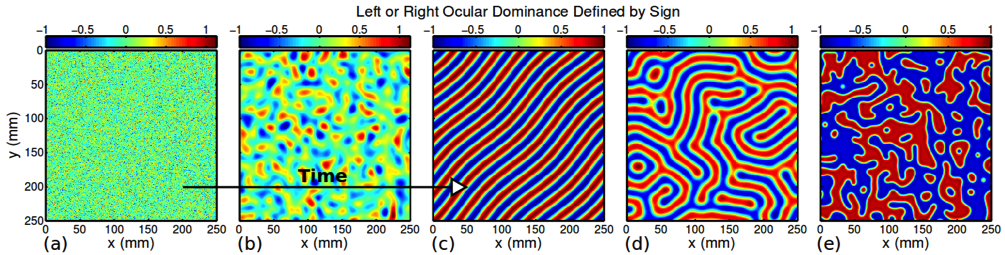
\includegraphics[width=.98\textwidth]{ocular_dominace.png}
  \caption{\label{centfig} Figure.}
\end{figure*}

\section{Conclusions}\label{conclusions}

A simple model suffices to study basic properties of ocular dominance
self-organization. Possibly, a combination with models for
self-organization in neighboring cortical layers would allow to
investigate higher organizational principles of the cortex
\cite{Reichl2012}, e.g.~the coordination between ocular dominance,
orientation, and cytochrome oxidase.

%%%%%%%%%%%%%%%%%%%%%%%%%%%%%%%%%%%%%%%%%%%%%%
%%                                          %%
%% Backmatter begins here                   %%
%%                                          %%
%%%%%%%%%%%%%%%%%%%%%%%%%%%%%%%%%%%%%%%%%%%%%%

\begin{backmatter}

\section*{Availability of Supporting Data}
More information about this project can be found at: \url{https://github.com/SOBF}. Further data and files supporting this project are hosted in the \emph{GigaScience} repository REFXXX.

\section*{Competing interests}
None

\section*{Author's contributions}
JPP, RM, LCTH, and DD performed the project and wrote the report.

\section*{Acknowledgements}
The authors would like to thank the organizers and attendees of the 2015
OHBM Hackathon. This work was supported by generous donations from
individuals to the Center for Investigating Healthy Minds, founded and
led by Dr.~Richard J. Davidson.

  
  
%%%%%%%%%%%%%%%%%%%%%%%%%%%%%%%%%%%%%%%%%%%%%%%%%%%%%%%%%%%%%
%%                  The Bibliography                       %%
%%                                                         %%
%%  Bmc_mathpys.bst  will be used to                       %%
%%  create a .BBL file for submission.                     %%
%%  After submission of the .TEX file,                     %%
%%  you will be prompted to submit your .BBL file.         %%
%%                                                         %%
%%                                                         %%
%%  Note that the displayed Bibliography will not          %%
%%  necessarily be rendered by Latex exactly as specified  %%
%%  in the online Instructions for Authors.                %%
%%                                                         %%
%%%%%%%%%%%%%%%%%%%%%%%%%%%%%%%%%%%%%%%%%%%%%%%%%%%%%%%%%%%%%

% if your bibliography is in bibtex format, use those commands:
\bibliographystyle{bmc-mathphys} % Style BST file
\bibliography{brainhack-report} % Bibliography file (usually '*.bib' )

\end{backmatter}
\end{document}
